\begin{figure}[!htbp]
\centering
\begin{tikzpicture}[schema base]
\node[schema esterno,text width=13.7cm] at (7.5,0)
  {\textbf{Filtro geometrico comune dopo l'assemblaggio}\\$\rho<0{,}02$: esclusione dall'uso previsto, non cancellazione dell'asset};
\node[schema titolo] at (0.3,-1.3) {Immagini: interpretazione generativa};
\node[schema titolo] at (8.1,-1.3) {Tabelle: trasformazione deterministica};
\draw[schema separatore,draw=schemaGrigio!55] (7.5,-1.6) -- (7.5,-8.55);
\node[schema oggetto,minimum width=4.2cm,minimum height=2.5cm] (immagine) at (3.3,-2.85) {};
\node[inner sep=0pt] at (3.3,-2.6)
  {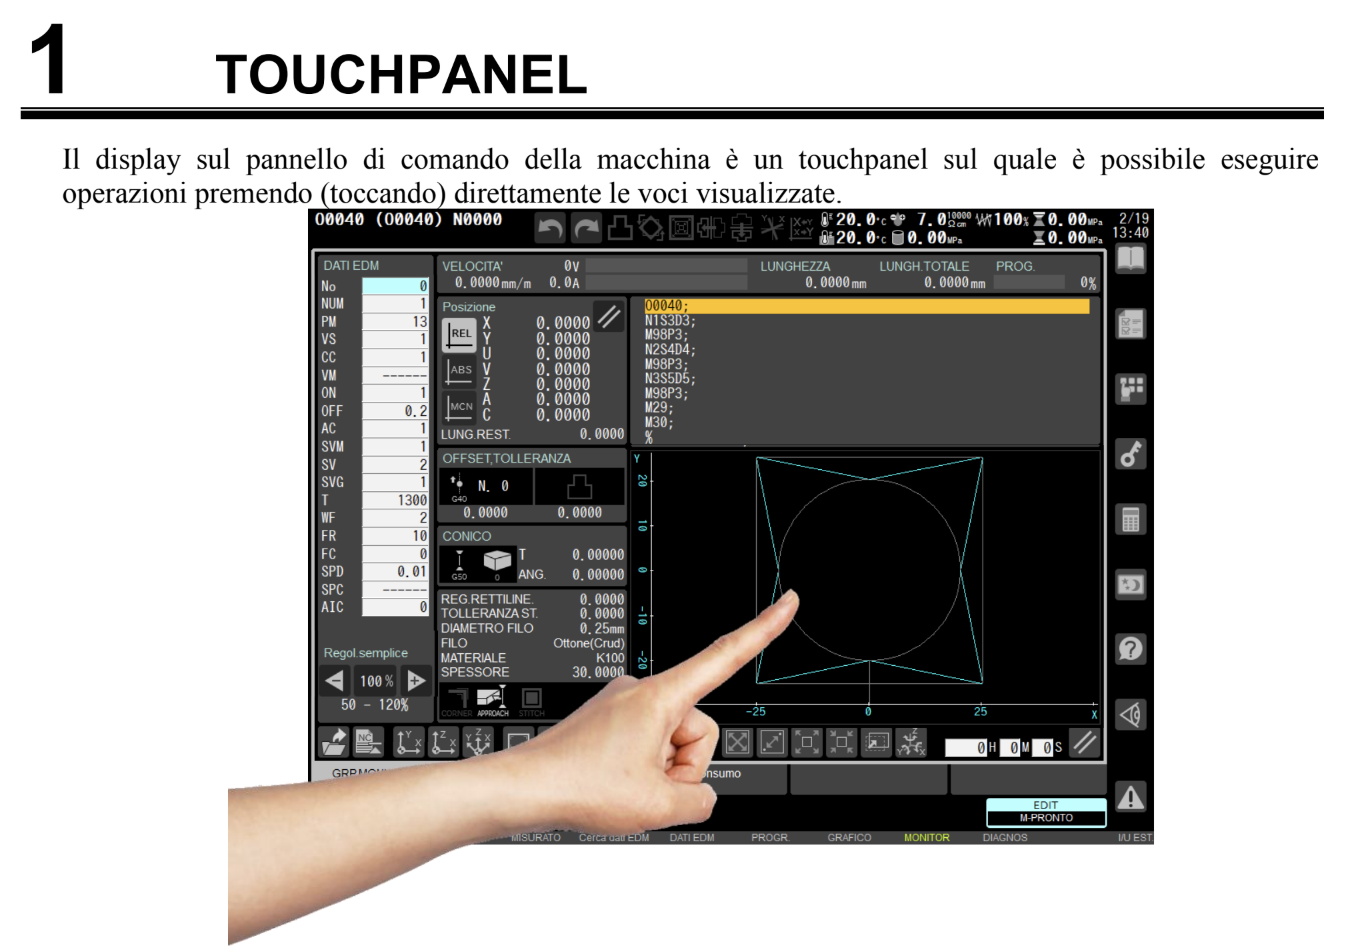
\includegraphics[width=3.7cm,height=2.15cm,keepaspectratio]{figure/asset/touch-panel-schermata-operatore.png}};
\node[schema nota,text width=6cm] at (3.3,-4.05) {Ritaglio ammissibile\\+ eventuale contesto sorgente};
\node[schema oggetto,minimum height=2.5cm] (tabella) at (11.7,-2.85) {};
\pic[scale=1.8] at (11.7,-2.6) {tabella};
\node[schema nota,text width=6cm] at (11.7,-4.05) {Contenuto testuale acquisito\\in Markdown o HTML};
\node[schema oggetto,minimum height=1.5cm] (caption) at (3.3,-5.65) {};
\pic[scale=0.72] at (2.35,-5.65) {modello};
\pic[scale=0.65] at (4.5,-5.65) {dialogo};
\draw[schema freccia] (3.1,-5.65) -- (3.73,-5.65);
\node[schema etichetta,text width=6.1cm] at (3.3,-7.55)
  {\textbf{Captioning con VLM}\\Controlli di formato e lunghezza;\\accettazione, revisione o errore.\\La fedeltà richiede verifica sulla fonte.};
\node[schema oggetto,minimum height=1.5cm] (righe) at (11.7,-5.65) {};
\foreach \ordinata/\colore in {-5.12/schemaBlu,-5.65/schemaVerde,-6.18/schemaOcra} {
  \path[schema icona,draw=\colore,fill=\colore!12] (9.5,\ordinata-0.19) rectangle (13.9,\ordinata+0.19);
  \node[font=\ttfamily\footnotesize] at (11.7,\ordinata) {intestazione: valore};
}
\node[schema etichetta,text width=6.1cm] at (11.7,-7.55)
  {\textbf{Serializzazione delle righe}\\Righe con contesto, testo di ripiego\\o contenuto non disponibile.\\Nessun valore non acquisito viene ricostruito.};
\draw[schema freccia] (3.3,-4.55) -- (caption.north);
\draw[schema freccia] (11.7,-4.55) -- (righe.north);
\end{tikzpicture}
\caption{Trattamento delle immagini e delle tabelle nel workflow corrente; le colonne non indicano esecuzione parallela. Schermata del manuale FANUC dai materiali forniti come esempio visuale, non risultato del captioning; tabella e righe sono schematiche. Le tabelle non vengono inviate al VLM e sono serializzate anche se escluse dall'uso previsto, senza annullare tale esclusione.}
\label{fig:trattamento-visuale}
\end{figure}